% Created 2022-10-12 Wed 16:32
% Intended LaTeX compiler: pdflatex
\documentclass[presentation,aspectratio=169, usenames, dvipsnames]{beamer}
\usepackage[utf8]{inputenc}
\usepackage[T1]{fontenc}
\usepackage{graphicx}
\usepackage{grffile}
\usepackage{longtable}
\usepackage{wrapfig}
\usepackage{rotating}
\usepackage[normalem]{ulem}
\usepackage{amsmath}
\usepackage{textcomp}
\usepackage{amssymb}
\usepackage{capt-of}
\usepackage{hyperref}
\usepackage{khpreamble}
\usepackage{amssymb}
\usepgfplotslibrary{groupplots}
\newcommand*{\shift}{\operatorname{q}}
\definecolor{ppc}{rgb}{0.1,0.1,0.6}
\definecolor{iic}{rgb}{0.6,0.1,0.1}
\definecolor{ddc}{rgb}{0.1,0.6,0.1}
\usetikzlibrary{positioning,circuits.plc.ladder}
\newcommand*{\coil}[1]{to[short] ++(0.5, 0) node[coordinate] (orig) {} arc [start angle=180, end angle=150,radius=8mm] (orig) arc [start angle=180, end angle=210,radius=8mm] (orig) ++(1cm, 0) node[coordinate] (coilend) {} arc [start angle=0, end angle=30,radius=8mm] (coilend) arc [start angle=0, end angle=-30,radius=8mm] (coilend) to[short] ++(0.5cm, 0) (orig) ++(0.5, 0.8) node {#1}}
\usetheme{default}
\author{Kjartan Halvorsen}
\date{\today}
\title{Sistemas de control y automatización}
\hypersetup{
 pdfauthor={Kjartan Halvorsen},
 pdftitle={Sistemas de control y automatización},
 pdfkeywords={},
 pdfsubject={},
 pdfcreator={Emacs 26.3 (Org mode 9.4.6)}, 
 pdflang={English}}
\begin{document}

\maketitle

\section{Ceneval}
\label{sec:org9507565}

\begin{frame}[label={sec:org396b593}]{CENEVAL}
\begin{center}
  \includegraphics[width=.7\linewidth]{./subareas.png}
\end{center}
\end{frame}

\begin{frame}[label={sec:org4e6e0e8}]{CENEVAL}
\begin{center}
  \includegraphics[width=.7\linewidth]{./seccion-D.png}
\end{center}
\end{frame}


\section{Feedback}
\label{sec:org46ff7e9}

\begin{frame}[label={sec:orgff4b0ff}]{Sistemas de control son ubicuos}
\begin{center}
  \includegraphics[width=.6\linewidth]{../figures/PnID-ex.png}
\end{center}
\end{frame}


\begin{frame}[label={sec:org1ab27c7}]{Control en lazo cerrado}
\begin{center}
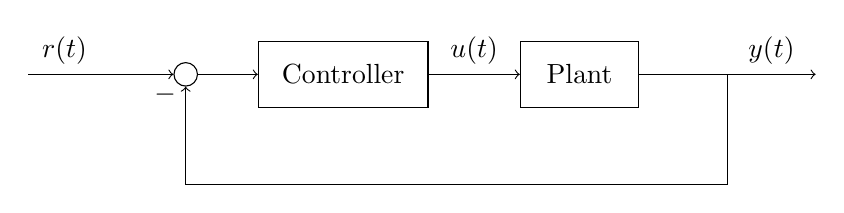
\begin{tikzpicture}[node distance=20mm,
                    block/.style={rectangle, draw, minimum width=15mm, inner sep=3mm},
                    sumnode/.style={circle, draw, inner sep=3pt}]
  \node[coordinate] (input) {};
  \node[sumnode, right of=input] (sum) {};
   \node[block, right of=sum,] (lti) {Controller};
   \node[block, right of=lti, node distance=30mm] (lti2) {Plant};
   \node[coordinate, right of=lti2, node distance=30mm] (output) {};
   \draw[->] (input) -- node[near start, above] {$r(t)$}  (sum);
   \draw[->] (sum) -- node[ above] {}  (lti);
   \draw[->] (lti) -- node[ above] {$u(t)$}  (lti2);
   \draw[->] (lti2) -- node[coordinate] (meas) {} node[near end, above] {$y(t)$} (output);
   \draw[->] (meas) -- ++(0, -14mm) -| node[left, pos=0.96] {$-$} (sum);
 \end{tikzpicture}
\end{center}
\end{frame}


\begin{frame}[label={sec:org73174da}]{Control en lazo cerrado}
\begin{center}
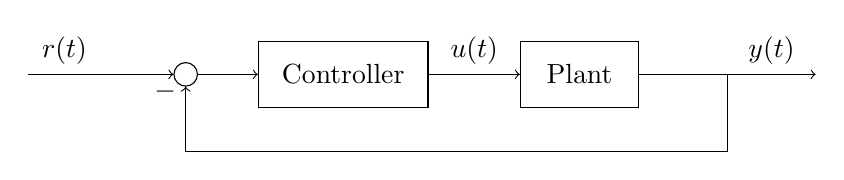
\begin{tikzpicture}[scale = 0.7, node distance=20mm,
                    block/.style={rectangle, draw, minimum width=15mm, inner sep=3mm},
                    sumnode/.style={circle, draw, inner sep=3pt}]
  \node[coordinate] (input) {};
  \node[sumnode, right of=input] (sum) {};
   \node[block, right of=sum,] (lti) {Controller};
   \node[block, right of=lti, node distance=30mm] (lti2) {Plant};
   \node[coordinate, right of=lti2, node distance=30mm] (output) {};
   \draw[->] (input) -- node[near start, above] {$r(t)$}  (sum);
   \draw[->] (sum) -- node[ above] {}  (lti);
   \draw[->] (lti) -- node[ above] {$u(t)$}  (lti2);
   \draw[->] (lti2) -- node[coordinate] (meas) {} node[near end, above] {$y(t)$} (output);
   \draw[->] (meas) -- ++(0, -14mm) -| node[left, pos=0.96] {$-$} (sum);
 \end{tikzpicture}
\end{center}

\alert{Diseño de control:} Determinar un controlador para que el sistema en lazo cerrado cumple con ciertas \alert{especificaciones de rendimiento}. 
\end{frame}

\begin{frame}[label={sec:org2a7c240}]{Especificaciones de rendimiento}
\begin{center}
  \includegraphics[width=.8\linewidth]{../figures/step-response-specifications}
\end{center}
\end{frame}


\begin{frame}[label={sec:org68b48da}]{Especificaciones de rendimiento}
\alert{Actividad} ¿Cumple el sistema con las especificaciones?

\begin{columns}
\begin{column}{0.4\columnwidth}
\begin{center}
\begin{tabular}{ll}
Sobreimpulso & < 20\%\\
Tiempo de levantamiento & < 1.5s\\
\end{tabular}
\end{center}
\end{column}


\begin{column}{0.6\columnwidth}
\begin{center}
 \includegraphics[width=1.0\linewidth]{../figures/second-order-response-example}
\end{center}
\end{column}
\end{columns}
\end{frame}



\section{Modeling}
\label{sec:org3e35a2f}
\begin{frame}[label={sec:org4b03f83}]{Sistemas de primer orden}
\begin{center}
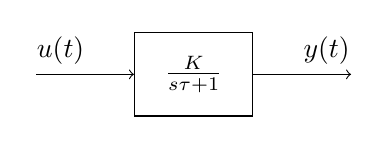
\begin{tikzpicture}[node distance=20mm,
                    block/.style={rectangle, draw, minimum width=15mm, inner sep=3mm},
                    sumnode/.style={circle, draw, inner sep=3pt}]
  \node[coordinate] (input) {};
   \node[block, right of=input,] (lti) {$\frac{K}{s\tau + 1}$};
   \node[coordinate, right of=lti, node distance=20mm] (output) {};
   \draw[->] (input) -- node[near start, above] {$u(t)$}  (lti);
   \draw[->] (lti) -- node[coordinate] (meas) {} node[near end, above] {$y(t)$} (output);
 \end{tikzpicture}
\end{center}
\end{frame}



\begin{frame}[label={sec:org3941995}]{Respuesta al escalón por medio de la transformada de Laplace}
\begin{block}{Parametrizaciónes alternativas}
\[ \frac{d}{dt} y + \alpha y = \beta u  \qquad \Leftrightarrow \qquad \tau \frac{d}{dt} y + y = k u \]
\end{block}
\end{frame}



\begin{frame}[label={sec:org971bf07}]{Función de transferencia por prueba}
\[  \quad \textcolor{green!50!black}{Y(s)} = \frac{K}{s\tau + 1}\textcolor{blue!80!black}{U(s)} \quad \overset{U(s) = \frac{u_f}{s}}{\Longrightarrow} \quad \textcolor{green!50!black}{y(t)} = u_f K\big( 1 - \mathrm{e}^{-\frac{t}{\tau}}\big)u_H(t)\]
\def\Tcnst{3}
\def\tdelay{0.0}
\def\ggain{2}
\def\uampl{0.8}
\pgfmathsetmacro{\yfinal}{\uampl*\ggain}
\pgfmathsetmacro{\yone}{0.283*\yfinal}
\pgfmathsetmacro{\ytwo}{0.632*\yfinal}
\pgfmathsetmacro{\tone}{\tdelay + \Tcnst/3}
\pgfmathsetmacro{\two}{\tdelay + \Tcnst}

\begin{center}
  \begin{tikzpicture}
    \begin{axis}[
    width=14cm,
    height=4.5cm,
    grid = both,
    xtick = {0,  \two},
    xticklabels = {0, $\tau$},
    ytick = {0, \ytwo, \uampl, \yfinal},
    yticklabels = {0,  $ $, $u_f$, $y_f$},
    xmin = -0.2,
    %minor y tick num=9,
    %minor x tick num=9,
    %every major grid/.style={red, opacity=0.5},
    xlabel = {$t$},
    ]
      \addplot [thick, green!50!black, no marks, domain=0:10, samples=100] {\uampl*\ggain*(x>\tdelay)*(1 - exp(-(x-\tdelay)/\Tcnst)} node [coordinate, pos=0.9, pin=-90:{$y(t)$}] {};
      \addplot [const plot, thick, blue!80!black, no marks, domain=-1:10, samples=100] coordinates {(-1,0) (0,0) (0,\uampl) (10,\uampl)} node [coordinate, pos=0.9, pin=-90:{$u(t)$}] {};
    \end{axis}
  \end{tikzpicture}
\end{center}

\alert{Actividad} Evalua la respuesta \(y(t)\) por \(t=\tau\),  y por \(t\to\infty\)!
\end{frame}

\begin{frame}[label={sec:org0519dc8}]{Función de transferencia por prueba}
\[  \quad \textcolor{green!50!black}{Y(s)} = \frac{K}{s\tau + 1}\textcolor{blue!80!black}{U(s)} \quad \overset{U(s) = \frac{u_f}{s}}{\Longrightarrow} \quad \textcolor{green!50!black}{y(t)} = u_f K\big( 1 - \mathrm{e}^{-\frac{t}{\tau}}\big)u_H(t)\]
\def\Tcnst{3}
\def\tdelay{0.0}
\def\ggain{2}
\def\uampl{0.8}
\pgfmathsetmacro{\yfinal}{\uampl*\ggain}
\pgfmathsetmacro{\yone}{0.283*\yfinal}
\pgfmathsetmacro{\ytwo}{0.632*\yfinal}
\pgfmathsetmacro{\tone}{\tdelay + \Tcnst/3}
\pgfmathsetmacro{\two}{\tdelay + \Tcnst}

\begin{center}
  \small
  \begin{tikzpicture}
    \begin{axis}[
    width=14cm,
    height=3.5cm,
    grid = both,
    xtick = {0,  \two},
    xticklabels = {0, $\tau$},
    ytick = {0, \ytwo, \uampl, \yfinal},
    yticklabels = {0,  $0.632y_f$, $u_f$, $y_f$},
    xmin = -0.2,
    %minor y tick num=9,
    %minor x tick num=9,
    %every major grid/.style={red, opacity=0.5},
    xlabel = {$t$},
    ]
      \addplot [thick, green!50!black, no marks, domain=0:10, samples=100] {\uampl*\ggain*(x>\tdelay)*(1 - exp(-(x-\tdelay)/\Tcnst)} node [coordinate, pos=0.9, pin=-90:{$y(t)$}] {};
      \addplot [const plot, thick, blue!80!black, no marks, domain=-1:10, samples=100] coordinates {(-1,0) (0,0) (0,\uampl) (10,\uampl)} node [coordinate, pos=0.9, pin=-90:{$u(t)$}] {};
    \end{axis}
  \end{tikzpicture}
\end{center}

\alert{Constante de tiempo:} El tiempo \(t=\tau\) que tarde la respuesta en llegar a 63.2\% del valor final.

\alert{Ganancia:} \(y_f = \lim_{t\to\infty}y(t) = Ku_f \quad \Rightarrow \quad K = \frac{y_f}{u_f}\)
\end{frame}

\begin{frame}[label={sec:org93f3223}]{Animación}
\href{https://kjartan-at-tec.github.io/mr2023/time-response-3.svg}{Sistemas de primer orden}
\end{frame}


\begin{frame}[label={sec:org5843f2d}]{Sistemas de primer orden con retraso}
\begin{center}
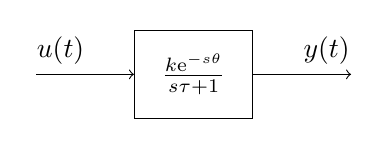
\begin{tikzpicture}[node distance=20mm,
                    block/.style={rectangle, draw, minimum width=15mm, inner sep=3mm},
                    sumnode/.style={circle, draw, inner sep=3pt}]
  \node[coordinate] (input) {};
   \node[block, right of=input,] (lti) {$\frac{k\mathrm{e}^{-s\theta}}{s\tau + 1}$};
   \node[coordinate, right of=lti, node distance=20mm] (output) {};
   \draw[->] (input) -- node[near start, above] {$u(t)$}  (lti);
   \draw[->] (lti) -- node[coordinate] (meas) {} node[anchor=west,near end, above] {$y(t)$} (output);
 \end{tikzpicture}
\end{center}
\end{frame}

\begin{frame}[label={sec:org82cebd2}]{Intermezzo: La función de transferencia de un retraso}
\begin{center}
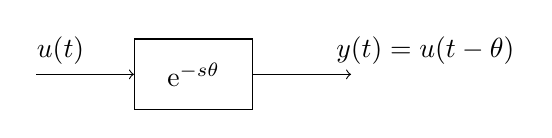
\begin{tikzpicture}[node distance=20mm,
                    block/.style={rectangle, draw, minimum width=15mm, inner sep=3mm},
                    sumnode/.style={circle, draw, inner sep=3pt}]
  \node[coordinate] (input) {};
   \node[block, right of=input,] (lti) {$\mathrm{e}^{-s\theta}$};
   \node[coordinate, right of=lti, node distance=20mm] (output) {};
   \draw[->] (input) -- node[near start, above] {$u(t)$}  (lti);
   \draw[->] (lti) -- node[coordinate] (meas) {} node[near end, above, anchor=south west] {$y(t)=u(t-\theta)$} (output);
 \end{tikzpicture}
\end{center}

\[ Y(s) = \laplace{y(t)} = \int_0^\infty y(t) \mathrm{e}^{-st} dt \]
\end{frame}

\begin{frame}[label={sec:org275d36f}]{Función de transferencia por prueba}
Modelo de primer orden con constante de tiempo \(\tau\) y retraso \(\theta\)
\[  \quad \textcolor{green!50!black}{Y(s)} = \frac{K\mathrm{e}^{-s\theta}}{s\tau + 1}\textcolor{blue!80!black}{U(s)} \quad \overset{U(s) = \frac{u_f}{s}}{\Longrightarrow} \quad \textcolor{green!50!black}{y(t)} = u_f K\big( 1 - \mathrm{e}^{-\frac{t-\theta}{\tau}}\big)u_H(t-\theta)\]
\def\Tcnst{3}
\def\tdelay{0.6}
\def\ggain{2}
\def\uampl{0.8}
\pgfmathsetmacro{\yfinal}{\uampl*\ggain}
\pgfmathsetmacro{\yone}{0.283*\yfinal}
\pgfmathsetmacro{\ytwo}{0.632*\yfinal}
\pgfmathsetmacro{\tone}{\tdelay + \Tcnst/3}
\pgfmathsetmacro{\two}{\tdelay + \Tcnst}

\begin{center}
  \begin{tikzpicture}
    \begin{axis}[
    width=14cm,
    height=4.5cm,
    grid = both,
    xtick = {0, \tdelay, \tone, \two},
    xticklabels = {0, $\theta$, $\theta+\frac{\tau}{3}$, $\theta + \tau$},
    ytick = {0, \yone, \ytwo, \uampl, \yfinal},
    yticklabels = {0, $ $, $ $, $u_f$, $y_f$},
    xmin = -0.2,
    %minor y tick num=9,
    %minor x tick num=9,
    %every major grid/.style={red, opacity=0.5},
    xlabel = {$t$},
    ]
      \addplot [thick, green!50!black, no marks, domain=0:10, samples=100] {\uampl*\ggain*(x>\tdelay)*(1 - exp(-(x-\tdelay)/\Tcnst)} node [coordinate, pos=0.9, pin=-90:{$y(t)$}] {};
      \addplot [const plot, thick, blue!80!black, no marks, domain=-1:10, samples=100] coordinates {(-1,0) (0,0) (0,\uampl) (10,\uampl)} node [coordinate, pos=0.9, pin=-90:{$u(t)$}] {};
    \end{axis}
  \end{tikzpicture}
\end{center}

\alert{Actividad} Evalua la respuesta  \(y(t)\) por \(t=\theta + \frac{\tau}{3}\) y \(t=\theta + \tau\)!
\end{frame}


\begin{frame}[label={sec:org46609cf}]{Función de transferencia por prueba}
Modelo de primer orden con constante de tiempo \(\tau\) y retraso \(\theta\)
\[  \quad \textcolor{green!50!black}{Y(s)} = \frac{K\mathrm{e}^{-s\theta}}{s\tau + 1}\textcolor{blue!80!black}{U(s)} \quad \overset{U(s) = \frac{u_f}{s}}{\Longrightarrow} \quad \textcolor{green!50!black}{y(t)} = u_f K\big( 1 - \mathrm{e}^{-\frac{t-\theta}{\tau}}\big)u_H(t-\theta)\]
\def\Tcnst{3}
\def\tdelay{0.6}
\def\ggain{2}
\def\uampl{0.8}
\pgfmathsetmacro{\yfinal}{\uampl*\ggain}
\pgfmathsetmacro{\yone}{0.283*\yfinal}
\pgfmathsetmacro{\ytwo}{0.632*\yfinal}
\pgfmathsetmacro{\tone}{\tdelay + \Tcnst/3}
\pgfmathsetmacro{\two}{\tdelay + \Tcnst}

\begin{center}
  \begin{tikzpicture}
    \begin{axis}[
    width=14cm,
    height=4.5cm,
    grid = both,
    xtick = {0, \tdelay, \tone, \two},
    xticklabels = {0, $\theta$, $\theta+\frac{\tau}{3}$, $\theta + \tau$},
    ytick = {0, \yone, \ytwo, \uampl, \yfinal},
    yticklabels = {0, $0.283y_{f}$, $0.632y_f$, $u_f$, $y_f$},
    xmin = -0.2,
    %minor y tick num=9,
    %minor x tick num=9,
    %every major grid/.style={red, opacity=0.5},
    xlabel = {$t$},
    ]
      \addplot [thick, green!50!black, no marks, domain=0:10, samples=100] {\uampl*\ggain*(x>\tdelay)*(1 - exp(-(x-\tdelay)/\Tcnst)} node [coordinate, pos=0.9, pin=-90:{$y(t)$}] {};
      \addplot [const plot, thick, blue!80!black, no marks, domain=-1:10, samples=100] coordinates {(-1,0) (0,0) (0,\uampl) (10,\uampl)} node [coordinate, pos=0.9, pin=-90:{$u(t)$}] {};
    \end{axis}
  \end{tikzpicture}
\end{center}

\[ y_f = \lim_{t\to\infty} y(t) = u_f K \quad \Rightarrow \quad K = \frac{y_f}{u_f}. \]
\end{frame}

\begin{frame}[label={sec:org25b7336}]{Función de transferencia por prueba - ejemplo}
\[  \quad Y(s) = \frac{K\mathrm{e}^{-s\theta}}{s\tau + 1}U(s) \quad \overset{U(s) = \frac{u_f}{s}}{\Longrightarrow} \quad y(t) = u_f K\big( 1 - \mathrm{e}^{-\frac{t-\theta}{\tau}}\big)u_s(t-\theta)\]
\def\Tcnst{2.1}
\def\tdelay{1}
\def\ggain{2}
\def\uampl{0.8}
\pgfmathsetmacro{\yfinal}{\uampl*\ggain}
\pgfmathsetmacro{\yone}{0.283*\yfinal}
\pgfmathsetmacro{\ytwo}{0.632*\yfinal}
\pgfmathsetmacro{\tone}{\tdelay + \Tcnst/3}
\pgfmathsetmacro{\two}{\tdelay + \Tcnst}

\begin{center}
  \begin{tikzpicture}
    \begin{axis}[
    width=12cm,
    height=4cm,
    grid = both,
    %xtick = {0, \tdelay, \tone, \two},
    %xticklabels = {0, $\theta$, $\theta+\frac{\tau}{3}$, $\theta + \tau$},
    %ytick = {0, \yone, \ytwo, \uampl, \yfinal},
    %yticklabels = {0, $0.283y_{f}$, $0.632y_f$, $u_f$, $y_f$},
    xmin = -0.2,
    minor y tick num=9,
    minor x tick num=9,
    every major grid/.style={red, opacity=0.5},
    %xlabel = {$t$},
    clip = false,
    ]
      \addplot [thick, green!50!black, smooth, no marks, domain=0:10, samples=16] {\uampl*\ggain*(x>\tdelay)*(1 - exp(-(x-\tdelay)/\Tcnst)} node [coordinate, pos=0.9, pin=-90:{$y(t)$}] {};
      \addplot [const plot, thick, blue!80!black, no marks, domain=-1:10, samples=100] coordinates {(-1,0) (0,0) (0,\uampl) (10,\uampl)} node [coordinate, pos=0.9, pin=-90:{$u(t)$}] {};
      \draw[thick, green!70!black, dashed] (axis cs: 10, \yfinal) -- (axis cs: -1, \yfinal, -0.9) node[left, anchor=east] {$y_f = \yfinal$}; 
      \draw[blue!70!black, dashed] (axis cs: 0, \uampl) -- (axis cs: -1, \uampl, -0.9) node[left, anchor=east] {$u_f = \uampl$}; 
    \end{axis}
  \end{tikzpicture}
\end{center}
\end{frame}

\begin{frame}[label={sec:org539b3f5}]{Función de transferencia por prueba - ejemplo}
\[  \quad Y(s) = \frac{K\mathrm{e}^{-s\theta}}{s\tau + 1}U(s) \quad \overset{U(s) = \frac{u_f}{s}}{\Longrightarrow} \quad y(t) = u_f K\big( 1 - \mathrm{e}^{-\frac{t-\theta}{\tau}}\big)u_s(t-\theta)\]
\def\Tcnst{2.1}
\def\tdelay{1}
\def\ggain{2}
\def\uampl{0.8}
\pgfmathsetmacro{\yfinal}{\uampl*\ggain}
\pgfmathsetmacro{\yone}{0.283*\yfinal}
\pgfmathsetmacro{\ytwo}{0.632*\yfinal}
\pgfmathsetmacro{\tone}{\tdelay + \Tcnst/3}
\pgfmathsetmacro{\two}{\tdelay + \Tcnst}

\begin{center}
  \begin{tikzpicture}
    \begin{axis}[
    width=12cm,
    height=4cm,
    grid = both,
    %xtick = {0, \tdelay, \tone, \two},
    %xticklabels = {0, $\theta$, $\theta+\frac{T}{3}$, $\theta + T$},
    %ytick = {0, \yone, \ytwo, \uampl, \yfinal},
    %yticklabels = {0, $0.283y_{f}$, $0.632y_f$, $u_f$, $y_f$},
    xmin = -0.2,
    minor y tick num=9,
    minor x tick num=9,
    every major grid/.style={red, opacity=0.5},
    %xlabel = {$t$},
    clip = false,
    ]
      \addplot [thick, green!50!black, smooth, no marks, domain=0:10, samples=16] {\uampl*\ggain*(x>\tdelay)*(1 - exp(-(x-\tdelay)/\Tcnst)} node [coordinate, pos=0.9, pin=-90:{$y(t)$}] {};
      \addplot [const plot, thick, blue!80!black, no marks, domain=-1:10, samples=100] coordinates {(-1,0) (0,0) (0,\uampl) (10,\uampl)} node [coordinate, pos=0.9, pin=-90:{$u(t)$}] {};
      \draw[thick, orange, dashed] (axis cs: \two, \ytwo) -- (axis cs: \two, -0.9) node[below] {$t_2 = \two = \theta + \tau$}; 
      \draw[thick, orange, dashed] (axis cs: \two, \ytwo) -- (axis cs: -1, \ytwo, -0.9) node[left, anchor=east] {$0.632y_f = \ytwo$}; 
      \draw[thick, green!70!black, dashed] (axis cs: 10, \yfinal) -- (axis cs: -1, \yfinal, -0.9) node[left, anchor=east] {$y_f = \yfinal$}; 
      \draw[blue!70!black, dashed] (axis cs: 0, \uampl) -- (axis cs: -1, \uampl, -0.9) node[left, anchor=east] {$u_f = \uampl$}; 
    \end{axis}
  \end{tikzpicture}
\end{center}
\end{frame}

\begin{frame}[label={sec:org096d1a3}]{Función de transferencia por prueba - ejemplo}
\[  \quad Y(s) = \frac{K\mathrm{e}^{-s\theta}}{s\tau + 1}U(s) \quad \overset{U(s) = \frac{u_f}{s}}{\Longrightarrow} \quad y(t) = u_f K\big( 1 - \mathrm{e}^{-\frac{t-\theta}{\tau}}\big)u_s(t-\theta)\]
\def\Tcnst{2.1}
\def\tdelay{1}
\def\ggain{2}
\def\uampl{0.8}
\pgfmathsetmacro{\yfinal}{\uampl*\ggain}
\pgfmathsetmacro{\yone}{0.283*\yfinal}
\pgfmathsetmacro{\ytwo}{0.632*\yfinal}
\pgfmathsetmacro{\tone}{\tdelay + \Tcnst/3}
\pgfmathsetmacro{\two}{\tdelay + \Tcnst}

\begin{center}
  \begin{tikzpicture}
    \begin{axis}[
    width=12cm,
    height=4cm,
    grid = both,
    %xtick = {0, \tdelay, \tone, \two},
    %xticklabels = {0, $\theta$, $\theta+\frac{T}{3}$, $\theta + T$},
    %ytick = {0, \yone, \ytwo, \uampl, \yfinal},
    %yticklabels = {0, $0.283y_{f}$, $0.632y_f$, $u_f$, $y_f$},
    xmin = -0.2,
    minor y tick num=9,
    minor x tick num=9,
    every major grid/.style={red, opacity=0.5},
    %xlabel = {$t$},
    clip = false,
    ]
      \addplot [thick, green!50!black, smooth, no marks, domain=0:10, samples=16] {\uampl*\ggain*(x>\tdelay)*(1 - exp(-(x-\tdelay)/\Tcnst)} node [coordinate, pos=0.9, pin=-90:{$y(t)$}] {};
      \addplot [const plot, thick, blue!80!black, no marks, domain=-1:10, samples=100] coordinates {(-1,0) (0,0) (0,\uampl) (10,\uampl)} node [coordinate, pos=0.9, pin=-90:{$u(t)$}] {};
      \draw[thick, red, dashed] (axis cs: \tone, \yone) -- (axis cs: \tone, -0.45) node[below] {$t_1 = \tone = \theta + \frac{\tau}{3}$}; 
      \draw[thick, red, dashed] (axis cs: \tone, \yone) -- (axis cs: -1,\yone) node[left, anchor=east] {$0.283y_f = \yone$}; 
      \draw[thick, orange, dashed] (axis cs: \two, \ytwo) -- (axis cs: \two, -0.9) node[below] {$t_2 = \two = \theta + \tau$}; 
      \draw[thick, orange, dashed] (axis cs: \two, \ytwo) -- (axis cs: -1, \ytwo, -0.9) node[left, anchor=east] {$0.632y_f = \ytwo$}; 
      \draw[thick, green!70!black, dashed] (axis cs: 10, \yfinal) -- (axis cs: -1, \yfinal, -0.9) node[left, anchor=east] {$y_f = \yfinal$}; 
      \draw[blue!70!black, dashed] (axis cs: 0, \uampl) -- (axis cs: -1, \uampl, -0.9) node[left, anchor=east] {$u_f = \uampl$}; 
    \end{axis}
  \end{tikzpicture}
\end{center}
\end{frame}

\begin{frame}[label={sec:org4b54423}]{Función de transferencia por prueba - ejemplo}
\[  \quad Y(s) = \frac{K\mathrm{e}^{-s\theta}}{s\tau + 1}U(s) \quad \overset{U(s) = \frac{u_f}{s}}{\Longrightarrow} \quad y(t) = u_f K\big( 1 - \mathrm{e}^{-\frac{t-\theta}{\tau}}\big)u_s(t-\theta)\]
\def\Tcnst{2.1}
\def\tdelay{1}
\def\ggain{2}
\def\uampl{0.8}
\pgfmathsetmacro{\yfinal}{\uampl*\ggain}
\pgfmathsetmacro{\yone}{0.283*\yfinal}
\pgfmathsetmacro{\ytwo}{0.632*\yfinal}
\pgfmathsetmacro{\tone}{\tdelay + \Tcnst/3}
\pgfmathsetmacro{\two}{\tdelay + \Tcnst}

\begin{center}
  \begin{tikzpicture}
    \begin{axis}[
    width=12cm,
    height=4cm,
    grid = both,
    %xtick = {0, \tdelay, \tone, \two},
    %xticklabels = {0, $\theta$, $\theta+\frac{T}{3}$, $\theta + T$},
    %ytick = {0, \yone, \ytwo, \uampl, \yfinal},
    %yticklabels = {0, $0.283y_{f}$, $0.632y_f$, $u_f$, $y_f$},
    xmin = -0.2,
    minor y tick num=9,
    minor x tick num=9,
    every major grid/.style={red, opacity=0.5},
    %xlabel = {$t$},
    clip = false,
    ]
      \addplot [thick, green!50!black, smooth, no marks, domain=0:10, samples=16] {\uampl*\ggain*(x>\tdelay)*(1 - exp(-(x-\tdelay)/\Tcnst)} node [coordinate, pos=0.9, pin=-90:{$y(t)$}] {};
      \addplot [const plot, thick, blue!80!black, no marks, domain=-1:10, samples=100] coordinates {(-1,0) (0,0) (0,\uampl) (10,\uampl)} node [coordinate, pos=0.9, pin=-90:{$u(t)$}] {};
      \draw[thick, red, dashed] (axis cs: \tone, \yone) -- (axis cs: \tone, -0.45) node[below] {$t_1 = \tone = \theta + \frac{\tau}{3}$}; 
      \draw[thick, red, dashed] (axis cs: \tone, \yone) -- (axis cs: -1,\yone) node[left, anchor=east] {$0.283y_f = \yone$}; 
      \draw[thick, orange, dashed] (axis cs: \two, \ytwo) -- (axis cs: \two, -0.9) node[below] {$t_2 = \two = \theta + \tau$}; 
      \draw[thick, orange, dashed] (axis cs: \two, \ytwo) -- (axis cs: -1, \ytwo, -0.9) node[left, anchor=east] {$0.632y_f = \ytwo$}; 
      \draw[thick, green!70!black, dashed] (axis cs: 10, \yfinal) -- (axis cs: -1, \yfinal, -0.9) node[left, anchor=east] {$y_f = \yfinal$}; 
      \draw[blue!70!black, dashed] (axis cs: 0, \uampl) -- (axis cs: -1, \uampl, -0.9) node[left, anchor=east] {$u_f = \uampl$}; 
    \end{axis}
  \end{tikzpicture}
\end{center}
\[ \begin{cases} \tone = \theta + \frac{\tau}{3}\\ \two = \theta + \tau \end{cases} \quad \Rightarrow \quad \begin{cases} \theta = \tdelay \\ \tau = \Tcnst \end{cases}, \qquad  K = \frac{y_f}{u_f} = \frac{\yfinal}{\uampl} = \ggain \]
\end{frame}


\begin{frame}[label={sec:org65c87d5}]{Sistemas de segundo orden}
\href{https://kjartan-at-tec.github.io/mr2023/time-response-4.svg}{Sistemas de segundo orden}
\end{frame}


\section{PID control}
\label{sec:orgf0bc7f0}

\begin{frame}[label={sec:orga32cfa2}]{PID control}
\end{frame}
\begin{frame}[label={sec:org87e1869}]{Control en lazo cerrado}
\begin{center}
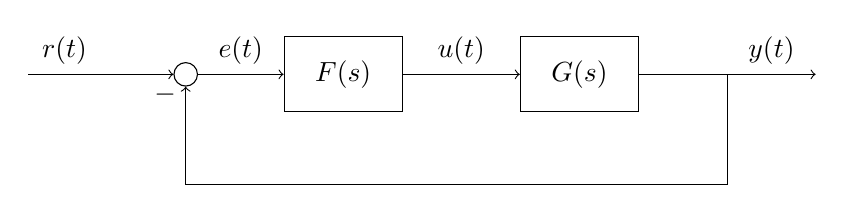
\begin{tikzpicture}[node distance=20mm,
                    block/.style={rectangle, draw, minimum width=15mm, inner sep=3mm},
                    sumnode/.style={circle, draw, inner sep=3pt}]
  \node[coordinate] (input) {};
  \node[sumnode, right of=input] (sum) {};
   \node[block, right of=sum,] (lti) {$F(s)$};
   \node[block, right of=lti, node distance=30mm] (lti2) {$G(s)$};
   \node[coordinate, right of=lti2, node distance=30mm] (output) {};
   \draw[->] (input) -- node[near start, above] {$r(t)$}  (sum);
   \draw[->] (sum) -- node[ above] {$e(t)$}  (lti);
   \draw[->] (lti) -- node[ above] {$u(t)$}  (lti2);
   \draw[->] (lti2) -- node[coordinate] (meas) {} node[near end, above] {$y(t)$} (output);
   \draw[->] (meas) -- ++(0, -14mm) -| node[left, pos=0.96] {$-$} (sum);
 \end{tikzpicture}
\end{center}
\end{frame}

\begin{frame}[label={sec:org46c446a}]{Controlador PID - Formas estándar}
\definecolor{ppc}{rgb}{0.1,0.1,0.6}
\definecolor{iic}{rgb}{0.6,0.1,0.1}
\definecolor{ddc}{rgb}{0.1,0.6,0.1}

\begin{center}
  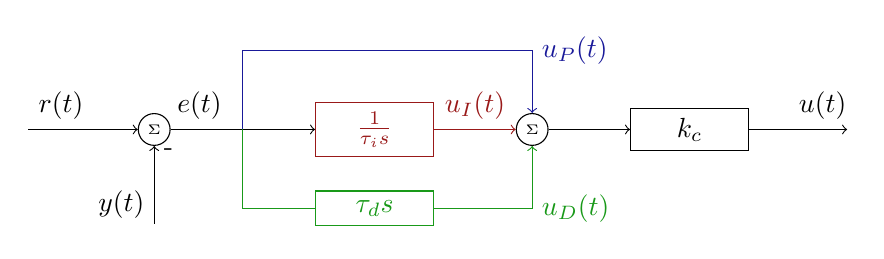
\begin{tikzpicture}[node distance=22mm, block/.style={rectangle, draw, minimum width=15mm}, sumnode/.style={circle, draw, inner sep=2pt}]

    \node[coordinate] (input) {};
    \node[sumnode, right of=input, node distance=16mm] (sum) {\tiny $\Sigma$};
    \node[color=iic,block, right of=sum, node distance=28mm] (ii)  {$\frac{1}{\tau_is}$};
    \node[color=ppc, coordinate, above of=ii, node distance=10mm] (pp)  {};
    \node[color=ddc,block, below of=ii, node distance=10mm] (dd)  {$\tau_ds$};
    \node[sumnode, right of=ii, node distance=20mm] (sum2) {\tiny $\Sigma$};
    \node[block, right of=sum2, node distance=20mm] (gain)  {$k_c$};
    \node[coordinate, below of=sum, node distance=12mm] (feedback) {};
    \node[coordinate, right of=gain, node distance=20mm] (output) {};

    \draw[->] (input) -- node[above, pos=0.3] {$r(t)$} (sum);
    \draw[->] (sum) -- node[above, pos=0.2] {$e(t)$} node[coordinate] (mm) {}  (ii);
    \draw[->] (gain) -- node[above, near end] {$u(t)$} (output);
    \draw[->] (feedback) -- node[left, near start] {$y(t)$} node[right, pos=0.95] {-} (sum);
    \draw[->, color=ppc] (mm) |- (pp) -| node[right,] {$u_P(t)$} (sum2);
    \draw[->, color=ddc] (mm) |- (dd) -| node[right,] {$u_D(t)$} (sum2);
    \draw[->, color=iic] (ii)  -- node[above,] {$u_I(t)$} (sum2);
    \draw[->] (sum2) -- node[above, near end] {} (gain);

  \end{tikzpicture}
\end{center}

\alert{ISA}
\begin{align*}
u(t) &= k_c\Big( \textcolor{ppc}{e(t)} + \textcolor{iic}{\frac{1}{\tau_i} \int_0^{t} e(\xi) d\xi} + \textcolor{ddc}{\tau_d \frac{d}{dt} e(t)} \Big)
\end{align*}

\alert{Paralela}
\begin{align*}
u(t) &=  \textcolor{ppc}{K_p e(t)} + \textcolor{iic}{K_i \int_0^{t} e(\xi) d\xi} + \textcolor{ddc}{K_d \frac{d}{dt} e(t)}
\end{align*}
\end{frame}

\begin{frame}[label={sec:orgf376ae1}]{Controlador PID}
\begin{center}
  \begin{tikzpicture}[node distance=22mm, block/.style={rectangle, draw, minimum width=15mm}, sumnode/.style={circle, draw, inner sep=2pt},scale=0.8, every node/.style={scale=0.8}]

    \node[coordinate] (input) {};
    \node[sumnode, right of=input, node distance=16mm] (sum) {\tiny $\Sigma$};
    \node[block, right of=sum, node distance=20mm] (pid)  {\textcolor{ppc}{P}\textcolor{iic}{I}\textcolor{ddc}{D}};
    \node[coordinate, below of=sum, node distance=12mm] (feedback) {};
    \node[coordinate, right of=pid, node distance=20mm] (output) {};

    \draw[->] (input) -- node[above, pos=0.3] {$r(t)$} (sum);
    \draw[->] (sum) -- node[above] {$e(t)$} (pid);
    \draw[->] (pid) -- node[above, near end] {$u(t)$} (output);
    \draw[->] (feedback) -- node[left, near start] {$y(t)$} node[right, pos=0.95] {-} (sum);

    \begin{scope}[yshift=-3cm]
    \foreach \pos/\clr/\nme in {0/ppc/P, 2/iic/I, 4/ddc/D} {
    \node (knob) at (\pos,0) {\includegraphics[width=12mm]{../figures/knob.png}};
    \node[above of=knob, node distance=10mm] {\large \textcolor{\clr}{\nme}};
    }
    \end{scope}

    \end{tikzpicture}
\end{center}

\pause

\begin{tabular}{lll}
\textbf{\textcolor{ppc}{P}} & Proporcional: & Modifica la velocidad del sistema de control\\
\textbf{\textcolor{iic}{I}} & Integral: & Elimina el error $e(t)$ en estado estable\\
\textbf{\textcolor{ddc}{D}} & Derivativa: & Mejora la amortiguación
\end{tabular}
\end{frame}

\begin{frame}[label={sec:orgfd823fc}]{Controlador PID - efecto de las ganancias}
Dado un sistema controlado por un PID \(U(s)=(K_P+K_I \frac{1}{s}+K_D s) E(s)\)
\begin{columns}
\begin{column}{0.7\columnwidth}
   \begin{center}
\includegraphics[width=0.48\linewidth]{../figures/fig930115-1a-1}
\includegraphics[width=0.48\linewidth]{../figures/fig930115-1a-2}\\
\includegraphics[width=0.48\linewidth]{../figures/fig930115-1a-3}
\includegraphics[width=0.48\linewidth]{../figures/fig930115-1a-4}
   \end{center}
\end{column}
\begin{column}{0.3\columnwidth}
Encuentra la respuesta del sistema en lazo cerrado para cada de los siguientes casos

\begin{center}
\begin{tabular}{lrrr}
Caso & \textcolor{ppc}{\(K_P\)} & \textcolor{iic}{\(K_I\)} & \textcolor{ddc}{\(K_D\)}\\
\hline
i) & 1 & 0 & 0\\
ii) & 1 & 1 & 0\\
iii) & 1 & 0 & 1\\
iv) & 1 & 1 & 1\\
\end{tabular}
\end{center}
\end{column}
\end{columns}
\end{frame}


\begin{frame}[label={sec:org0264335}]{Controlador PID - ajustar las ganancias}
\begin{columns}
\begin{column}{0.6\columnwidth}
\begin{center}
\includegraphics[width=0.99\linewidth]{../figures/stepresponse-secondorder-exercise}
\end{center}
\end{column}

\begin{column}{0.4\columnwidth}
\alert{Actividad} Cómo ajustar las ganancias \(K_P\), \(K_I\) y \(K_D\) para obtener una respuesta mejor?

\begin{center}
\begin{tabular}{llll}
Caso & \textcolor{ppc}{\(K_P\)} & \textcolor{iic}{\(K_I\)} & \textcolor{ddc}{\(K_D\)}\\
\hline
A &  &  & \\
B &  &  & \\
C &  &  & \\
D &  &  & \\
\hline
\end{tabular}
\end{center}
\end{column}
\end{columns}
\end{frame}

\section{PID tuning - (Smith and Corripio) Ziegler Nichols}
\label{sec:org46a0b4d}
\begin{frame}[label={sec:orge7e6974}]{Sintonización de controladores PID}
\alert{Hay varios métodos.} Entre otros:

\begin{itemize}
\item Ziegler \& Nichols método en lazo abierto,  y método en lazo cerrado
\item Smith \& Corripio (usando tabla de Ziegler \& Nichols)
\item Cohen \& Coon (como Smith \& Corripio, pero otros valores en la tabla)
\item Simple Internal Model Control (SIMC)
\end{itemize}
\end{frame}

\begin{frame}[label={sec:org519739a}]{Método de Smith \& Corripio con tabla de Ziegler \& Nichols}
\small

Dado modelo \[ G(s) = K \frac{\mathrm{e}^{-s\theta}}{\tau s + 1}, \] y controlador PID en forma
   \[ F(s) = k_c\left( 1 + \frac{1}{\tau_i s} + \tau_d s\right). \]

Elige los parámetros PID según la tabla siguiente (Ziegler \& Nichols, 1943)
   \begin{center}
   \setlength{\tabcolsep}{20pt}
   \renewcommand{\arraystretch}{1.5}
   \begin{tabular}{llll}
   Controller & \(k_c\) & \(\tau_i\) & \(\tau_d\)\\
  \hline\hline
  P & \(\frac{\tau}{\theta K}\) &  & \\
  PI & \(\frac{0.9\tau}{\theta K}\) & \(\frac{\theta}{0.3}\) & \\
  PID & \(\frac{1.2\tau}{\theta K}\) & \(2\theta\) & \(\frac{\theta}{2}\)\\
  \hline
\end{tabular}
\end{center}

Restricción: \[0.1 < \frac{\theta}{\tau} < 0.6.\]
\end{frame}


\begin{frame}[label={sec:orgb52f960}]{Método de Cohen \& Coon}
\small

Dado modelo \[ G(s) = K \frac{\mathrm{e}^{-s\theta}}{\tau s + 1}, \]
elige los parámetros PID según la tabla siguiente (Cohen \& Coon, 1953)
   \begin{center}
   \setlength{\tabcolsep}{20pt}
   \renewcommand{\arraystretch}{1.5}
   \begin{tabular}{llll}
   Controller & \(k_c\) & \(\tau_i\) & \(\tau_d\)\\
  \hline\hline
  P & \(\Big(1.03 + 0.35\big(\frac{\theta}{\tau}\big)\Big)\frac{\tau}{\theta K}\) &  & \\
  PI &  \(\Big(0.9 + 0.083\big(\frac{\theta}{\tau}\big)\Big)\frac{\tau}{\theta K}\) & \(\frac{\theta\Big(0.9 + 0.083\big(\frac{\theta}{\tau}\big)\Big)}{\Big(1.27 + 0.6\big(\frac{\theta}{\tau}\big)\Big)}\) & \\
  PID &  \(\Big(1.35 + 0.25\big(\frac{\theta}{\tau}\big)\Big)\frac{\tau}{\theta K}\) &  \(\frac{\theta\Big(1.35 + 0.25\big(\frac{\theta}{\tau}\big)\Big)}{\Big(0.54 + 0.33\big(\frac{\theta}{\tau}\big)\Big)}\) & \(\frac{\theta}{2\Big(1.35 + 0.25\big(\frac{\theta}{\tau}\big)\Big)}\)\\
  \hline
\end{tabular}
\end{center}
\end{frame}

\section{Digital logic}
\label{sec:org374183d}

\section{Automation}
\label{sec:org9cf8b86}
\begin{frame}[label={sec:orgcf6cbb0}]{Automatización}
\end{frame}
\begin{frame}[label={sec:org1137851}]{Automatización de un sistema neumático}
\begin{columns}
\begin{column}{0.3\columnwidth}
\begin{center}
 \includegraphics[width=1.0\linewidth]{../figures/fluidsim-32-solenoid-cylinder.png}
\end{center}
\end{column}
\begin{column}{0.6\columnwidth}
\pause

En la automatización de una prensa se requiere un pulsador para accionar un cilindro de simple efecto que permita sujetar una pieza metálica hasta que otro pulsador active el regreso del cilindro, liberando la pieza.
\end{column}
\end{columns}
\end{frame}

\begin{frame}[label={sec:orgb7cb80c}]{Automatizción de un sistema neumático}
\begin{columns}
\begin{column}{0.6\columnwidth}
Diagrama de escalera
\begin{center}
                 \begin{tikzpicture}[circuit plc ladder,]
                   \node at (1, -0.3) {?};
                   \node at (1, 0.2) {A};
                   \node at (3, -0.3) {?};
                   \node at (3, 0.2) {B};
                   \node at (1, -2) {?};
                   \node at (1, -1.5) {C};

                   \draw (0,0) to[short, o-]  (0,-4.5);
                   \draw (6,0) to[short, o-](6,-4.5);
                   \draw (0,-0.3) to[short, -o] (0.8, -0.3) (1.2, -0.3) to[short, o-]  (2,-0.3)
                    (2, -0.3) to[short, -o] (2.8, -0.3)
                    (3.2, -0.3) to[short, o-,] (4,-0.3) to[short] (4,-0.3) \coil{$K_1$};
                   \draw (0,-2) to[short, -o,] (0.8, -2)
                         (1.2, -2) to[short, o-,] (2,-2)  to[short] (2,-0.3);

                   \draw (0, -3.5) to[contact NO={info={$K_1$}},] (2, -3.5) to[short] (4, -3.5) \coil{Cylinder};
                 \end{tikzpicture}
\end{center}
\end{column}
\begin{column}{0.4\columnwidth}
\pause

Elementos de control

\begin{enumerate}
\item Pulsador NA
\item Pulsador NC
\item Contacto NA
\item Contacto NC
\end{enumerate}

Respuestas alternativas

\begin{enumerate}
\item A -- 1, B -- 2, C -- 3
\item A -- 2, B -- 4, C -- 3
\item A -- 1, B -- 2, C -- 4
\end{enumerate}
\end{column}
\end{columns}
\end{frame}

\begin{frame}[label={sec:orgda063de}]{¡Suerte!}
\Huge Lykke til!
\end{frame}
\end{document}